% Preamble
\documentclass[11pt]{article}

\title{Ethereum Payment Channel\\ECE 519C Project Report}
\author{Diyu Hu (V00968423)}

% Packages
\usepackage{amsmath}
\usepackage[a4paper, margin=2.5cm]{geometry}
\setlength\parindent{0pt}
\usepackage{verbatim}
\usepackage{graphicx}
\usepackage{wasysym}

% Document
\begin{document}
    \maketitle


    \section{Overview}\label{sec:overview}
    Payment channels allow participants to make repeated transfers of ether without using transactions.
    In this project, I will build a long-lived unidirectional payment channel between two participants.
    The usage of the proposed payment channel consist of:
    \begin{itemize}
        \item The sender opens a payment channel by deploys the smart contract with ether.
        \item The sender signs payment messages that specify the amount of ether owed to the receiver.
        \item The receiver closes the payment channel, withdrawing its authorized amount of ether and sending the
        remainder back to the sender.
        \item The sender adds more amount of ether to the smart contract.
        \item The receiver withdraws ether as needed before closing the channel.
        \item The sender initiates the closure of channel to retrieve unspent funds in a timeframe.
    \end{itemize}


    \section{Opening the Payment Channel}\label{sec:opening-the-payment-channel}
    To open a payment channel, the sender deploys the smart contract, attaching the amount of ether to be escrowed,
    specifying the intended receiver, and how long the receiver will have to close the channel after the sender
    initiates a close.
    \verbatiminput{./src/Opening-the-Payment-Channel.txt}


    \section{Making Payments}\label{sec:making-payments}
    The sender makes payments by sending messages to the receiver.
    Each message specifies a cumulative total amount of ether owed, rather than the amount of the individual
    micropayment.
    This step is preformed entirely outside the Ethereum network, e.g., using email or SMS (Short Message Service).
    Messages are cryptographically signed (e.g., using ECDSA) by the sender and then transmitted directly to the
    receiver.

    Each message consists of two parts:
    \begin{itemize}
        \item The address of the smart contract, which is used to prevent cross-contract replay attacks.
        \item The amount of ether owed to the receiver.
    \end{itemize}

    Payment messages can be constructed and signed in any language that supports cryptographic hashing and signing
    operations.
    The following example is written in JavaScript with Hardhat and Ethers:
    \verbatiminput{../scripts/SignPayment.js}
    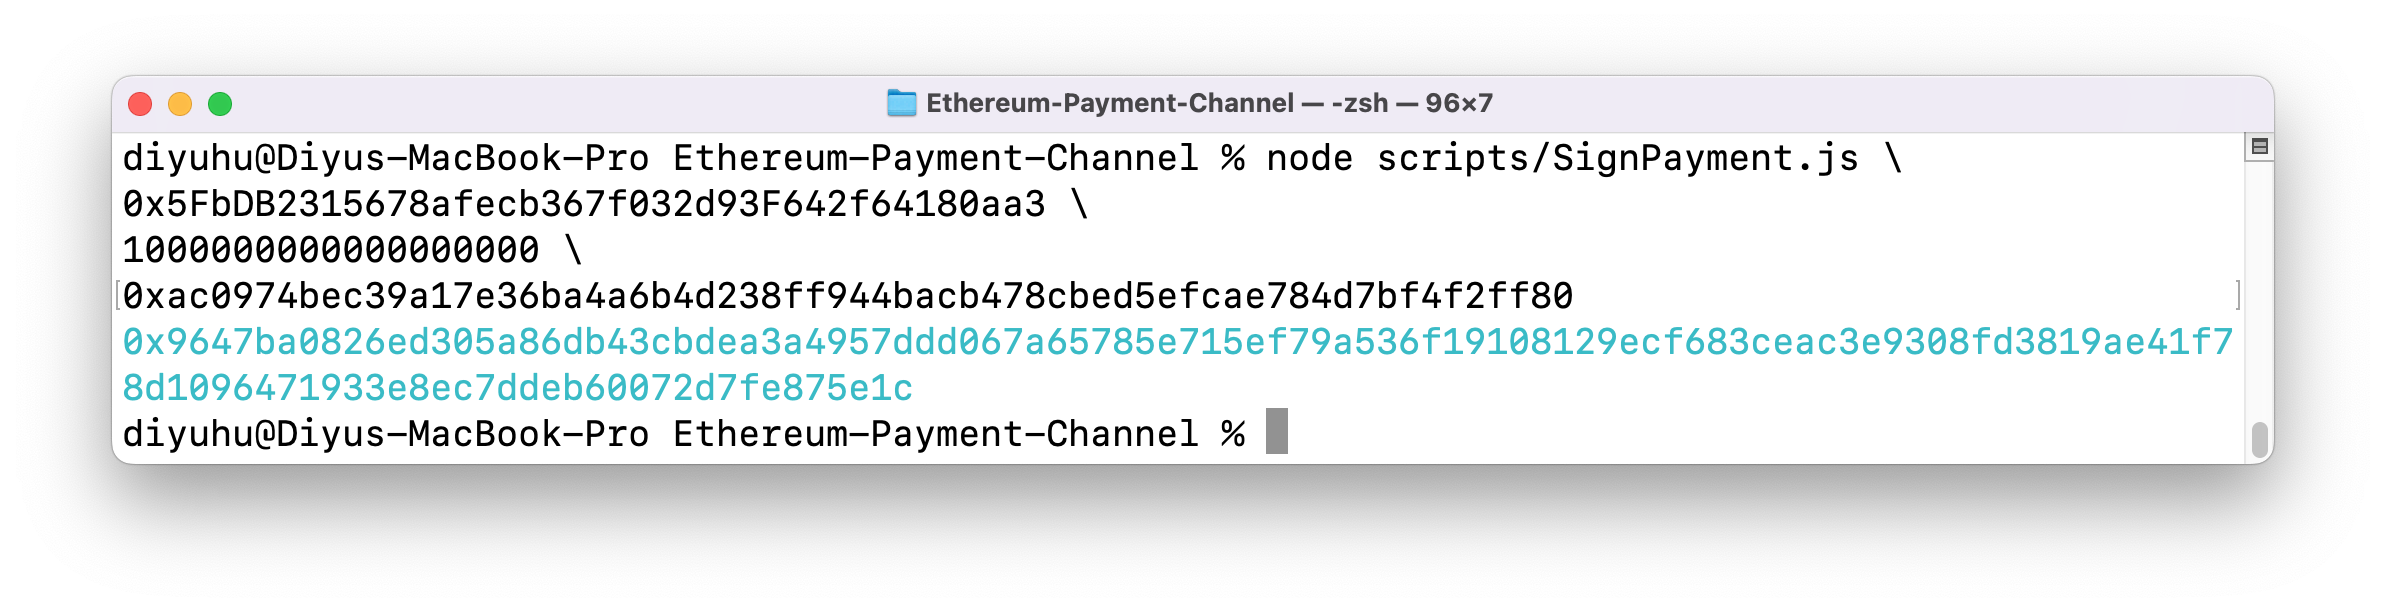
\includegraphics[width=\textwidth]{./images/sign-message-example}
    
    
    \section{Verify Payments}\label{sec:verify-payments}

\end{document}